\documentclass[11pt,letterpaper]{article}

\addtolength{\oddsidemargin}{-.875in}
\addtolength{\evensidemargin}{-.875in}
\addtolength{\textwidth}{1.75in}

\addtolength{\topmargin}{-.875in}
\addtolength{\textheight}{1.75in}

\usepackage[utf8]{inputenc}
\usepackage{caption} % for table captions
\usepackage{amsmath} % for multi-line equations and piecewises
\DeclareMathOperator{\sign}{sign}
\usepackage{graphicx}
\usepackage{relsize}
\usepackage{xspace}
\usepackage{verbatim} % for block comments
\usepackage{subcaption} % for subfigures
\usepackage{enumitem} % for a) b) c) lists
\newcommand{\Cyclus}{\textsc{Cyclus}\xspace}%
\newcommand{\Cycamore}{\textsc{Cycamore}\xspace}%
\newcommand{\deploy}{\texttt{d3ploy}\xspace}%
\newcommand{\Deploy}{\texttt{D3ploy}\xspace}%
\usepackage{tabularx}
\usepackage{color}
\usepackage{multirow}
\usepackage{float} 
\usepackage[acronym,toc]{glossaries}
%\include{acros}
\definecolor{bg}{rgb}{0.95,0.95,0.95}
\newcolumntype{b}{X}
\newcolumntype{f}{>{\hsize=.15\hsize}X}
\newcolumntype{s}{>{\hsize=.5\hsize}X}
\newcolumntype{m}{>{\hsize=.75\hsize}X}
\newcolumntype{r}{>{\hsize=1.1\hsize}X}
\usepackage{titling}
\usepackage[hang,flushmargin]{footmisc}
\renewcommand*\footnoterule{}
\usepackage{tikz}

\usetikzlibrary{shapes.geometric,arrows}
\tikzstyle{process} = [rectangle, rounded corners, 
minimum width=1cm, minimum height=1cm,text centered, draw=black, 
fill=blue!30]
\tikzstyle{arrow} = [thick,->,>=stealth]

\graphicspath{}
% \title{MHTGR350}
%\author{Roberto E. Fairhurst Agosta}

\begin{document}
%	\begin{titlepage}
%		\maketitle
%		\thispagestyle{empty}
%	\end{titlepage}

\section{OECD Exercise I}

oecd-exI-1b: 
Figure \ref{fig:compact}.
same material composition as OECD MHTGR 350 - Phase III

\begin{figure}[htbp!]
	\centering
	\includegraphics[height=5cm]{oecd-exI-1b1.png}
	\caption{Compact.}
	\label{fig:compact}
\end{figure}

\section{OECD Exercise II}

oecd-exI-2a: 
Figure \ref{fig:assembly}.

\begin{figure}[htbp!]
	\centering
	\includegraphics[height=5cm]{oecd-exI-2a.png}
	\caption{Fuel Assembly.}
	\label{fig:assembly}
\end{figure}

\section{OECD Standard-column}

Figure \ref{fig:stcol}.

\begin{figure}[htbp!]
	\centering
	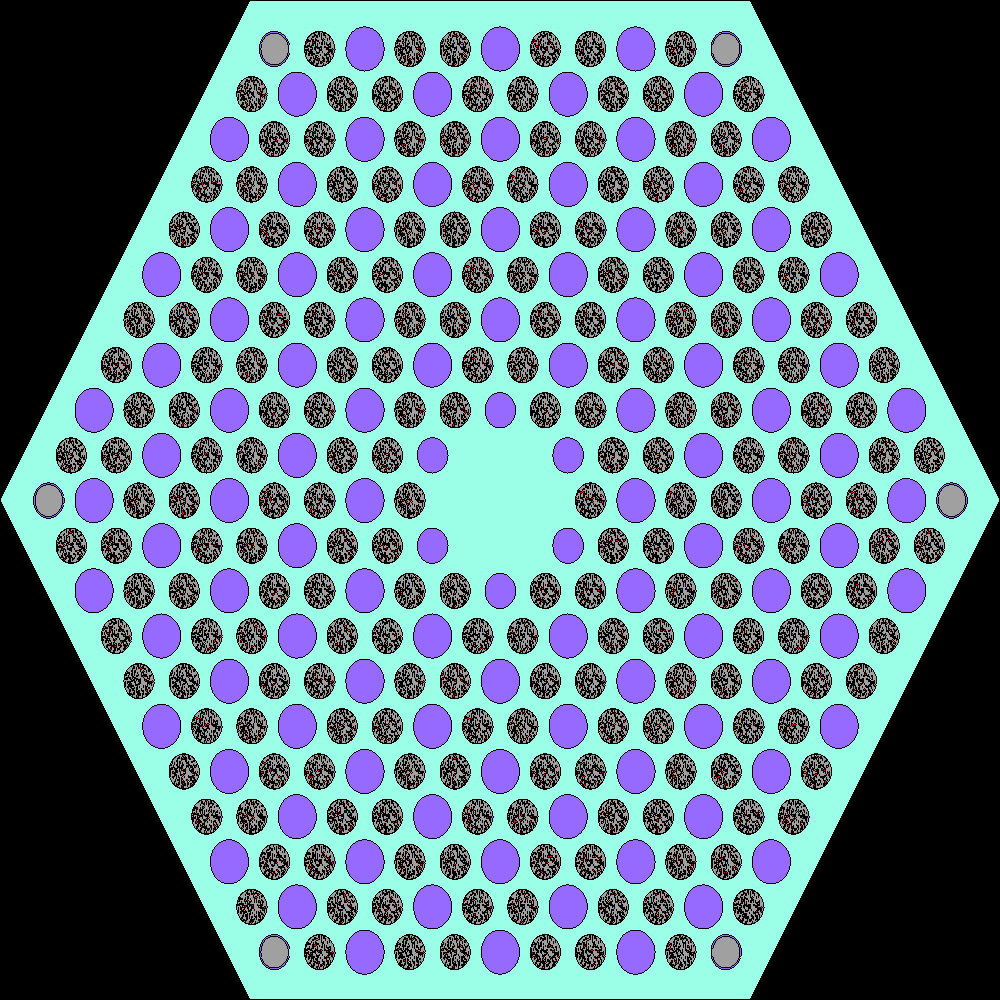
\includegraphics[height=5cm]{oecd-standard-column_geom1.png}
	\caption{Standard column.}
	\label{fig:stcol}
\end{figure}

\section{OECD Fullcore}

Figure \ref{fig:fullcore}.

\begin{figure}[htbp!]
	\centering
	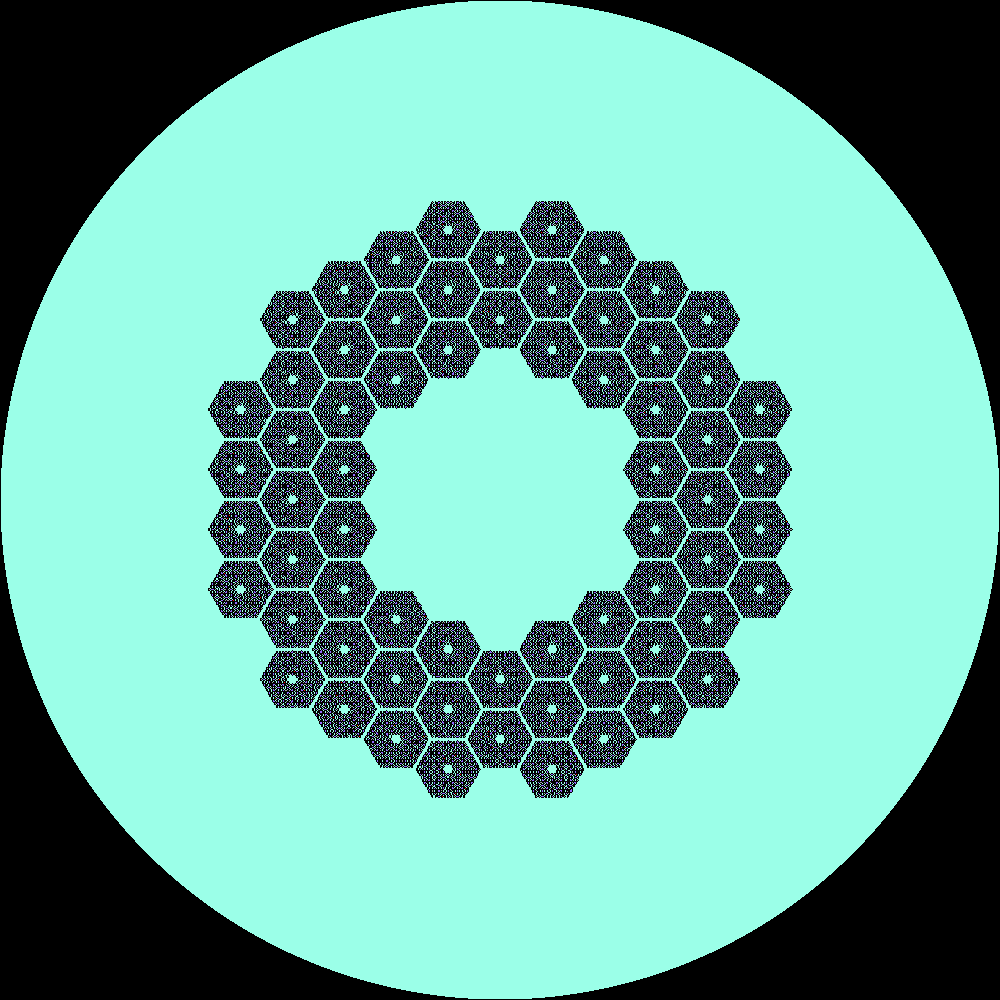
\includegraphics[height=5cm]{oecd-fullcore_geom1.png}
	\caption{Full core.}
	\label{fig:fullcore}
\end{figure}

\pagebreak
\bibliographystyle{plain}
\bibliography{bibliography}

\end{document}

	% \begin{table}[]
	% 	\centering
	%     \caption{TRISO and Fuel Compact Characteristics.}
	%     \label{tab:compact}
	% 	\begin{tabular}{l|l}
	% 	\hline
	% 	Characteristic                   & Value                \\ \hline
	% 	Fuel                             & UC$_{0.5}$O$_{1.5}$  \\
	% 	Enrichment (average)             & 15.5 wt\%            \\
	% 	Kernel radius                    & 0.02125 cm           \\
	% 	Buffer radius                    & 0.03125 cm           \\
	% 	IPyC radius                      & 0.03475 cm           \\
	% 	SiC radius                       & 0.03825 cm           \\
	% 	OPyC radius                      & 0.04225 cm           \\
	%  	Kernel density                   & 10.5 g/cm$^3$        \\
	% 	Buffer density                   & 1.0 g/cm$^3$         \\
	% 	IPyC density                     & 1.9 g/cm$^3$         \\
	% 	SiC density                      & 3.2 g/cm$^3$         \\
	% 	OPyC density                     & 1.9 g/cm$^3$         \\
	% 	Packing Fraction (average)       & 0.35                 \\
	% 	Compact radius                   & 0.6223 cm            \\
	% 	Compact Gap radius               & 0.635 cm             \\
	% 	Compact length                   & 4.928 cm             \\ 
	%   Helium density           		 & 4.19 kg/m$^3$        \\
	%   Block graphite density           & 1.85 g/cm$^3$        \\ \hline

	% 	\end{tabular}
	% \end{table}

	% \begin{figure}[htbp!]
	% 	\centering
	% 	\begin{subfigure}[t]{0.4\textwidth}
	% 		\centering
	% 		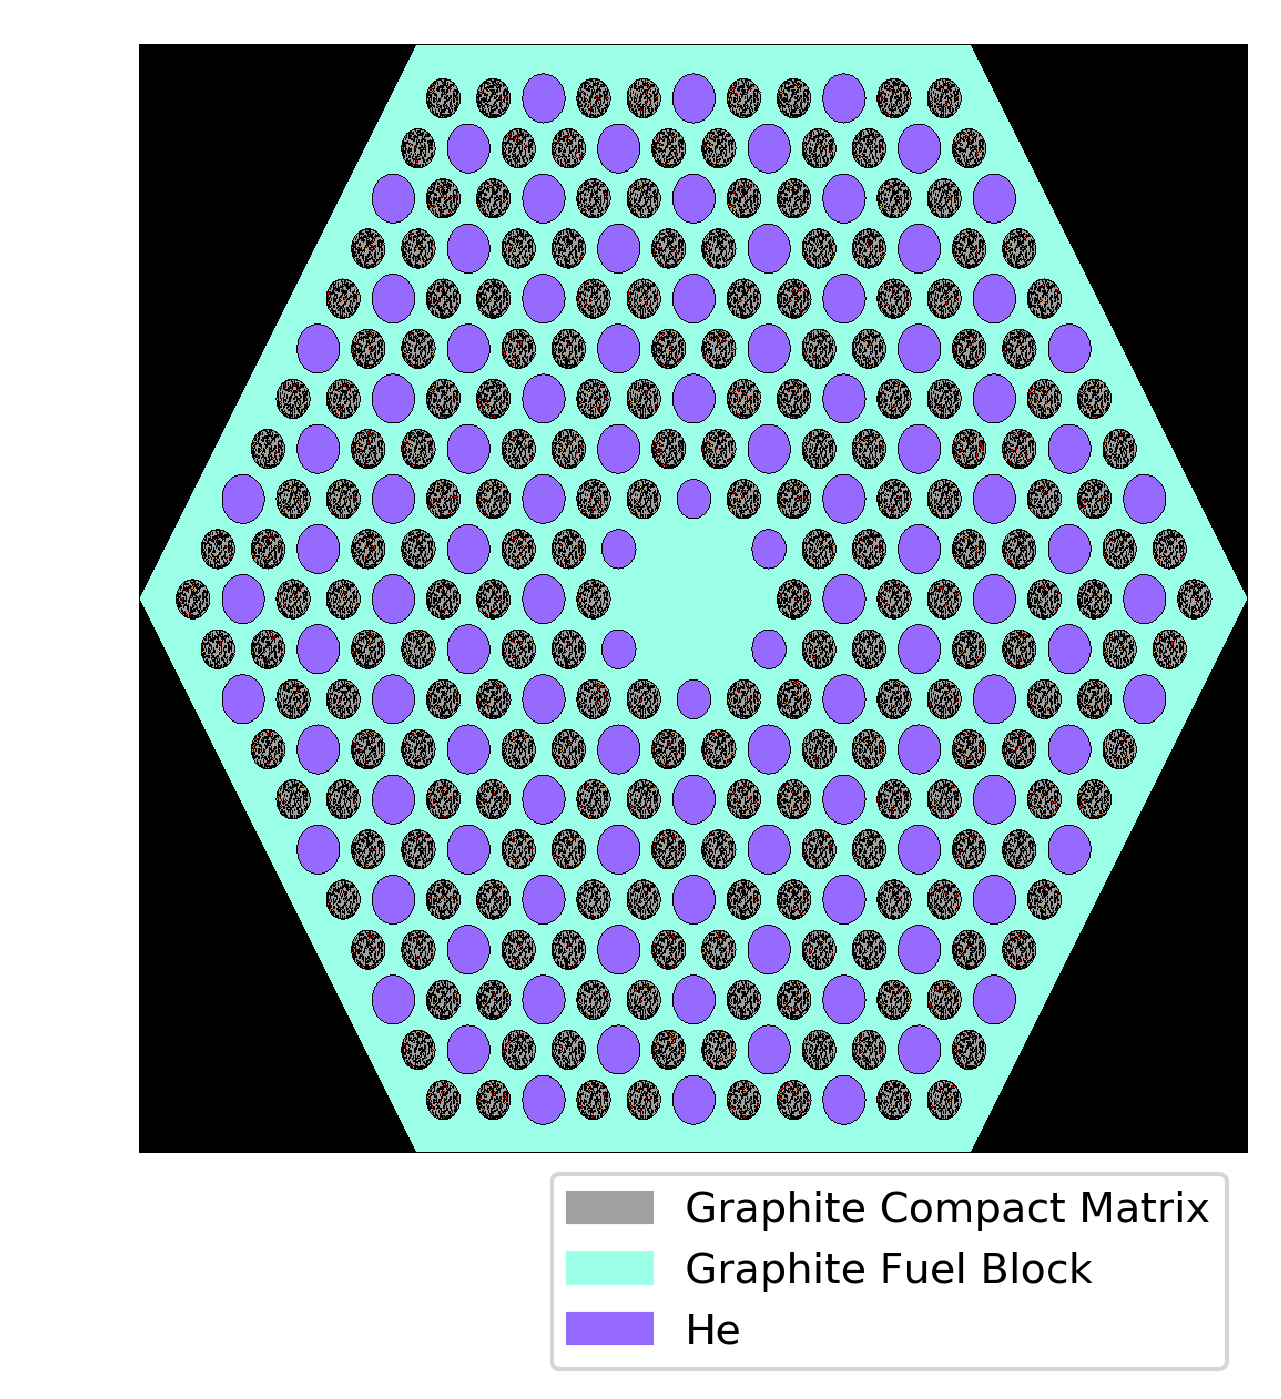
\includegraphics[width=\linewidth]{figures/standard.png}
	% 		\caption{XY-plane.}
	% 	\end{subfigure}
	% 	\begin{subfigure}[t]{0.4\textwidth}
	% 		\centering
	% 		\includegraphics[width=\linewidth]{figures/standard-column.png}
	% 		\caption{YZ-plane.}
	% 	\end{subfigure}
	% 	\hfill
	% 	\caption{Plot of \textit{standard-column}.}
	% 	\label{fig:standardcolumn}
	% \end{figure}

	% \begin{figure}[htbp!]
	% 	\centering
	% 	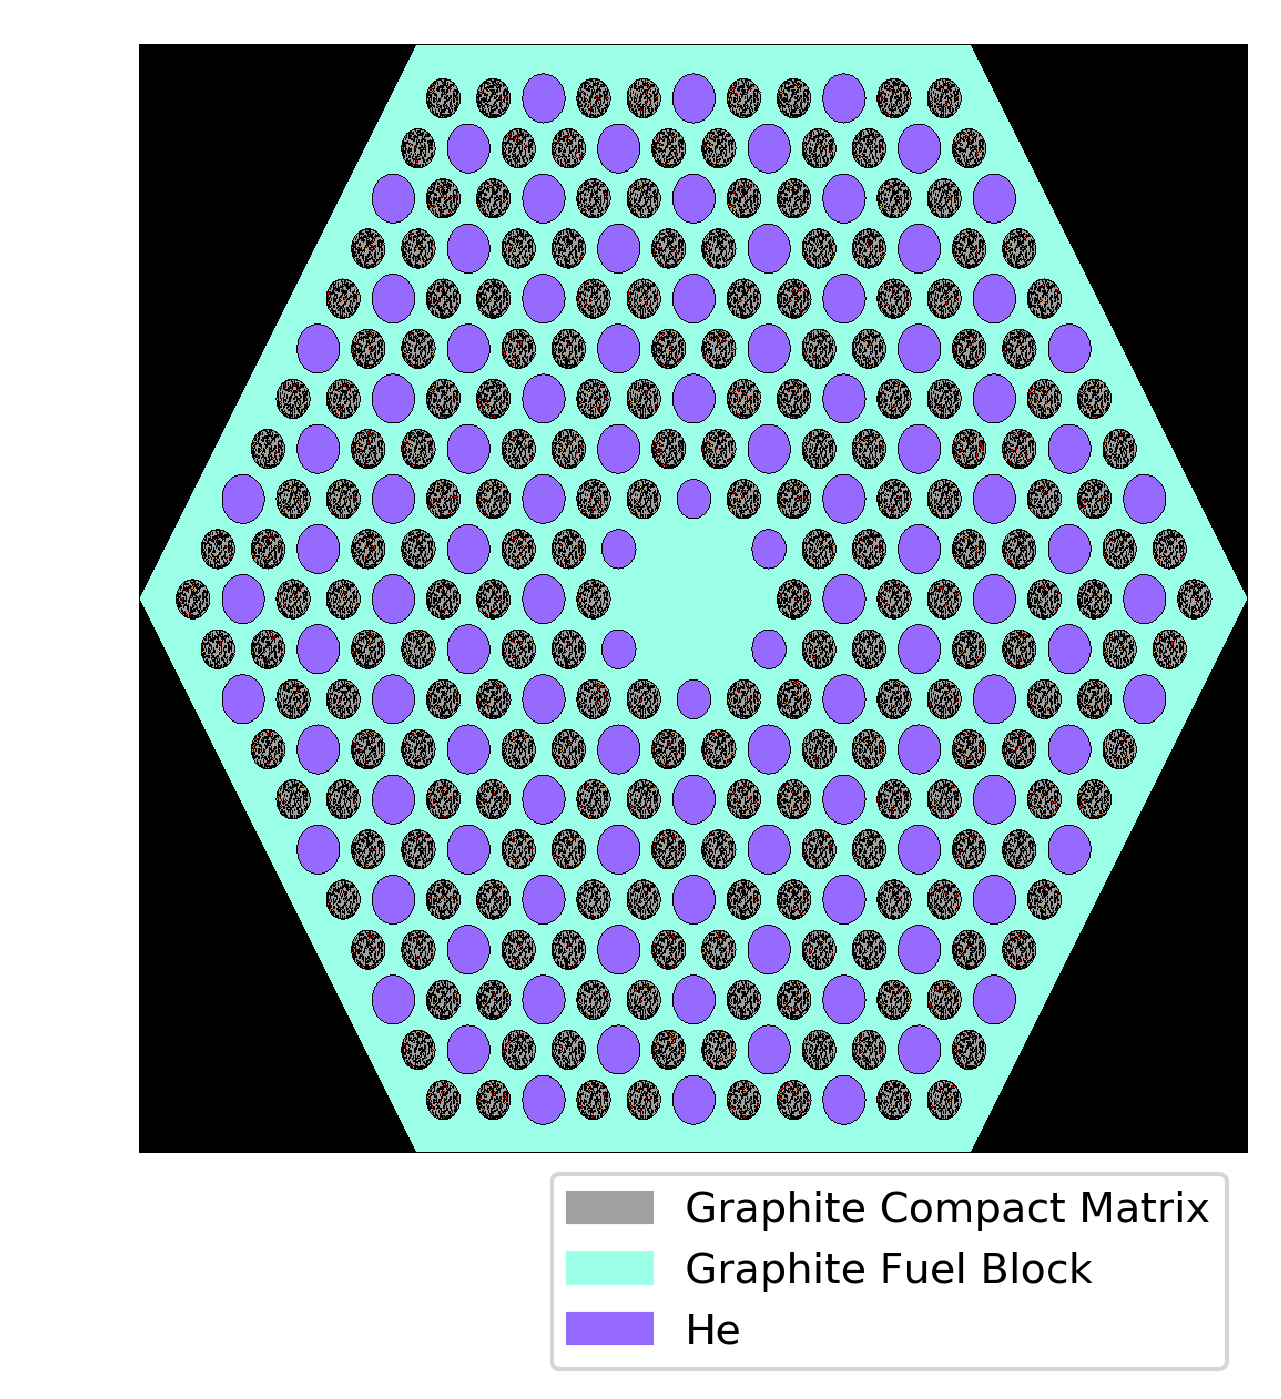
\includegraphics[height=5cm]{figures/standard.png}
	% 	\caption{Standard fuel assembly model.}
	% 	\label{fig:standard}
	% \end{figure}